\subsection{Data Description}

\subsection{...}
We evaluate the statistical properties of the resulting ocean forcing realizations by comparing it to the original simulation. We find that the forcing is realistic and that it captures the relevant spatial and temporal variability.

\begin{figure}
\centerline{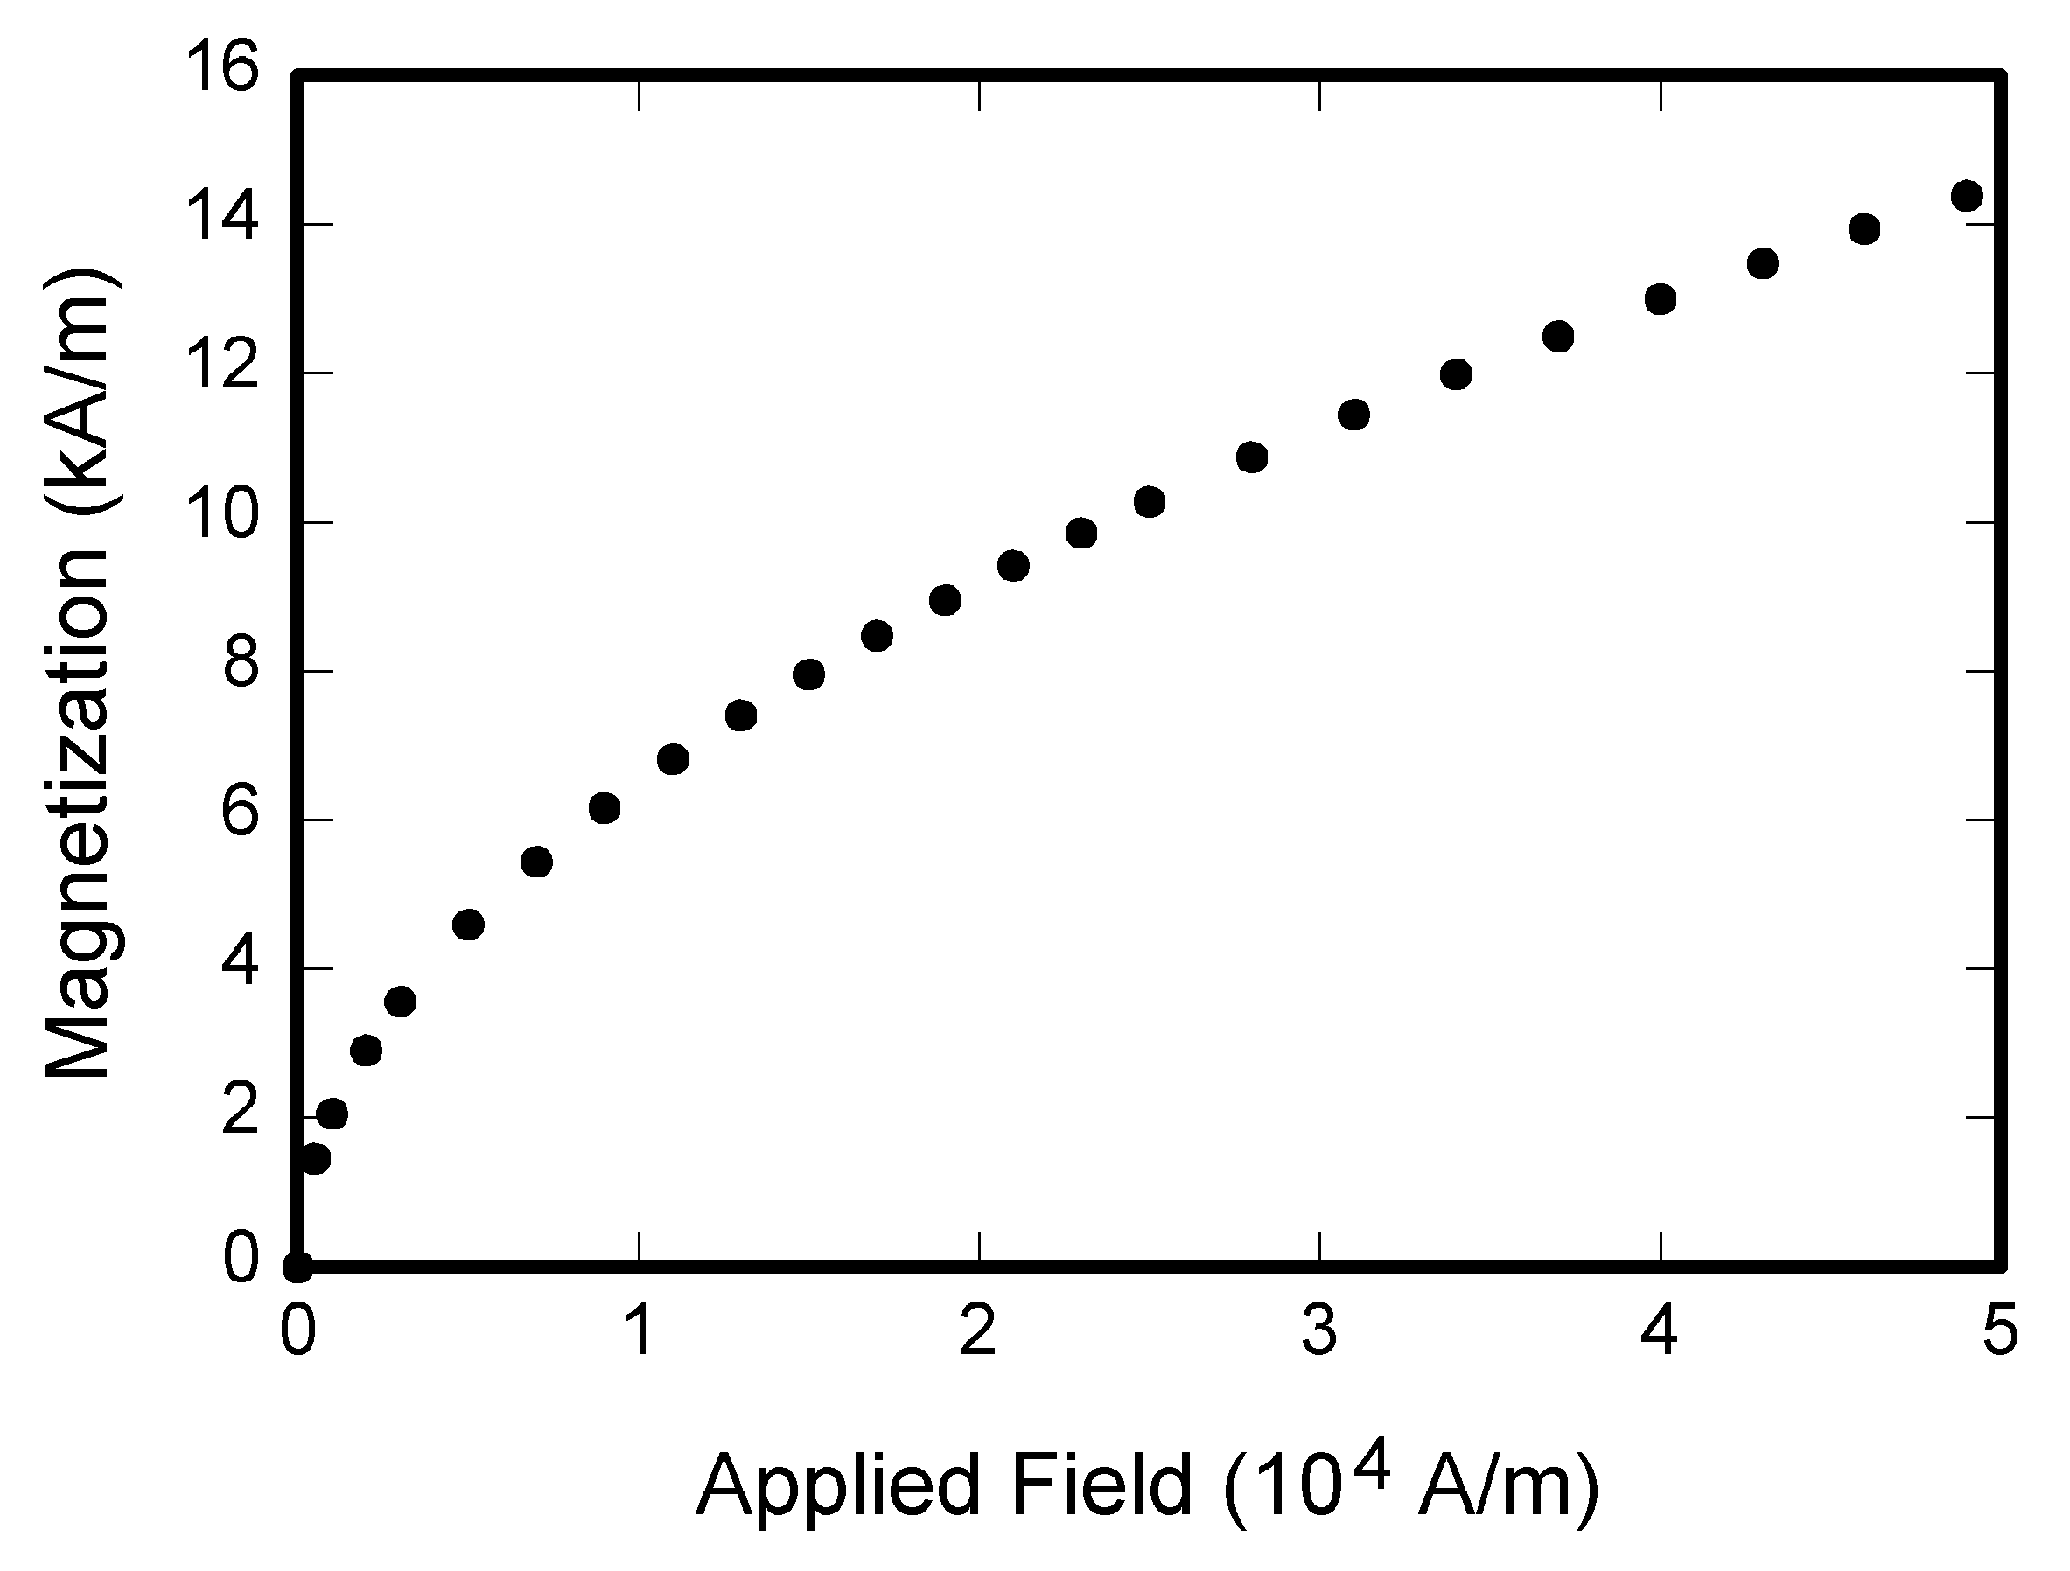
\includegraphics[width=18.5pc]{fig/fig1.png}}
\caption{Workflow / schematic of the generator}
\end{figure}

\begin{figure}
\centerline{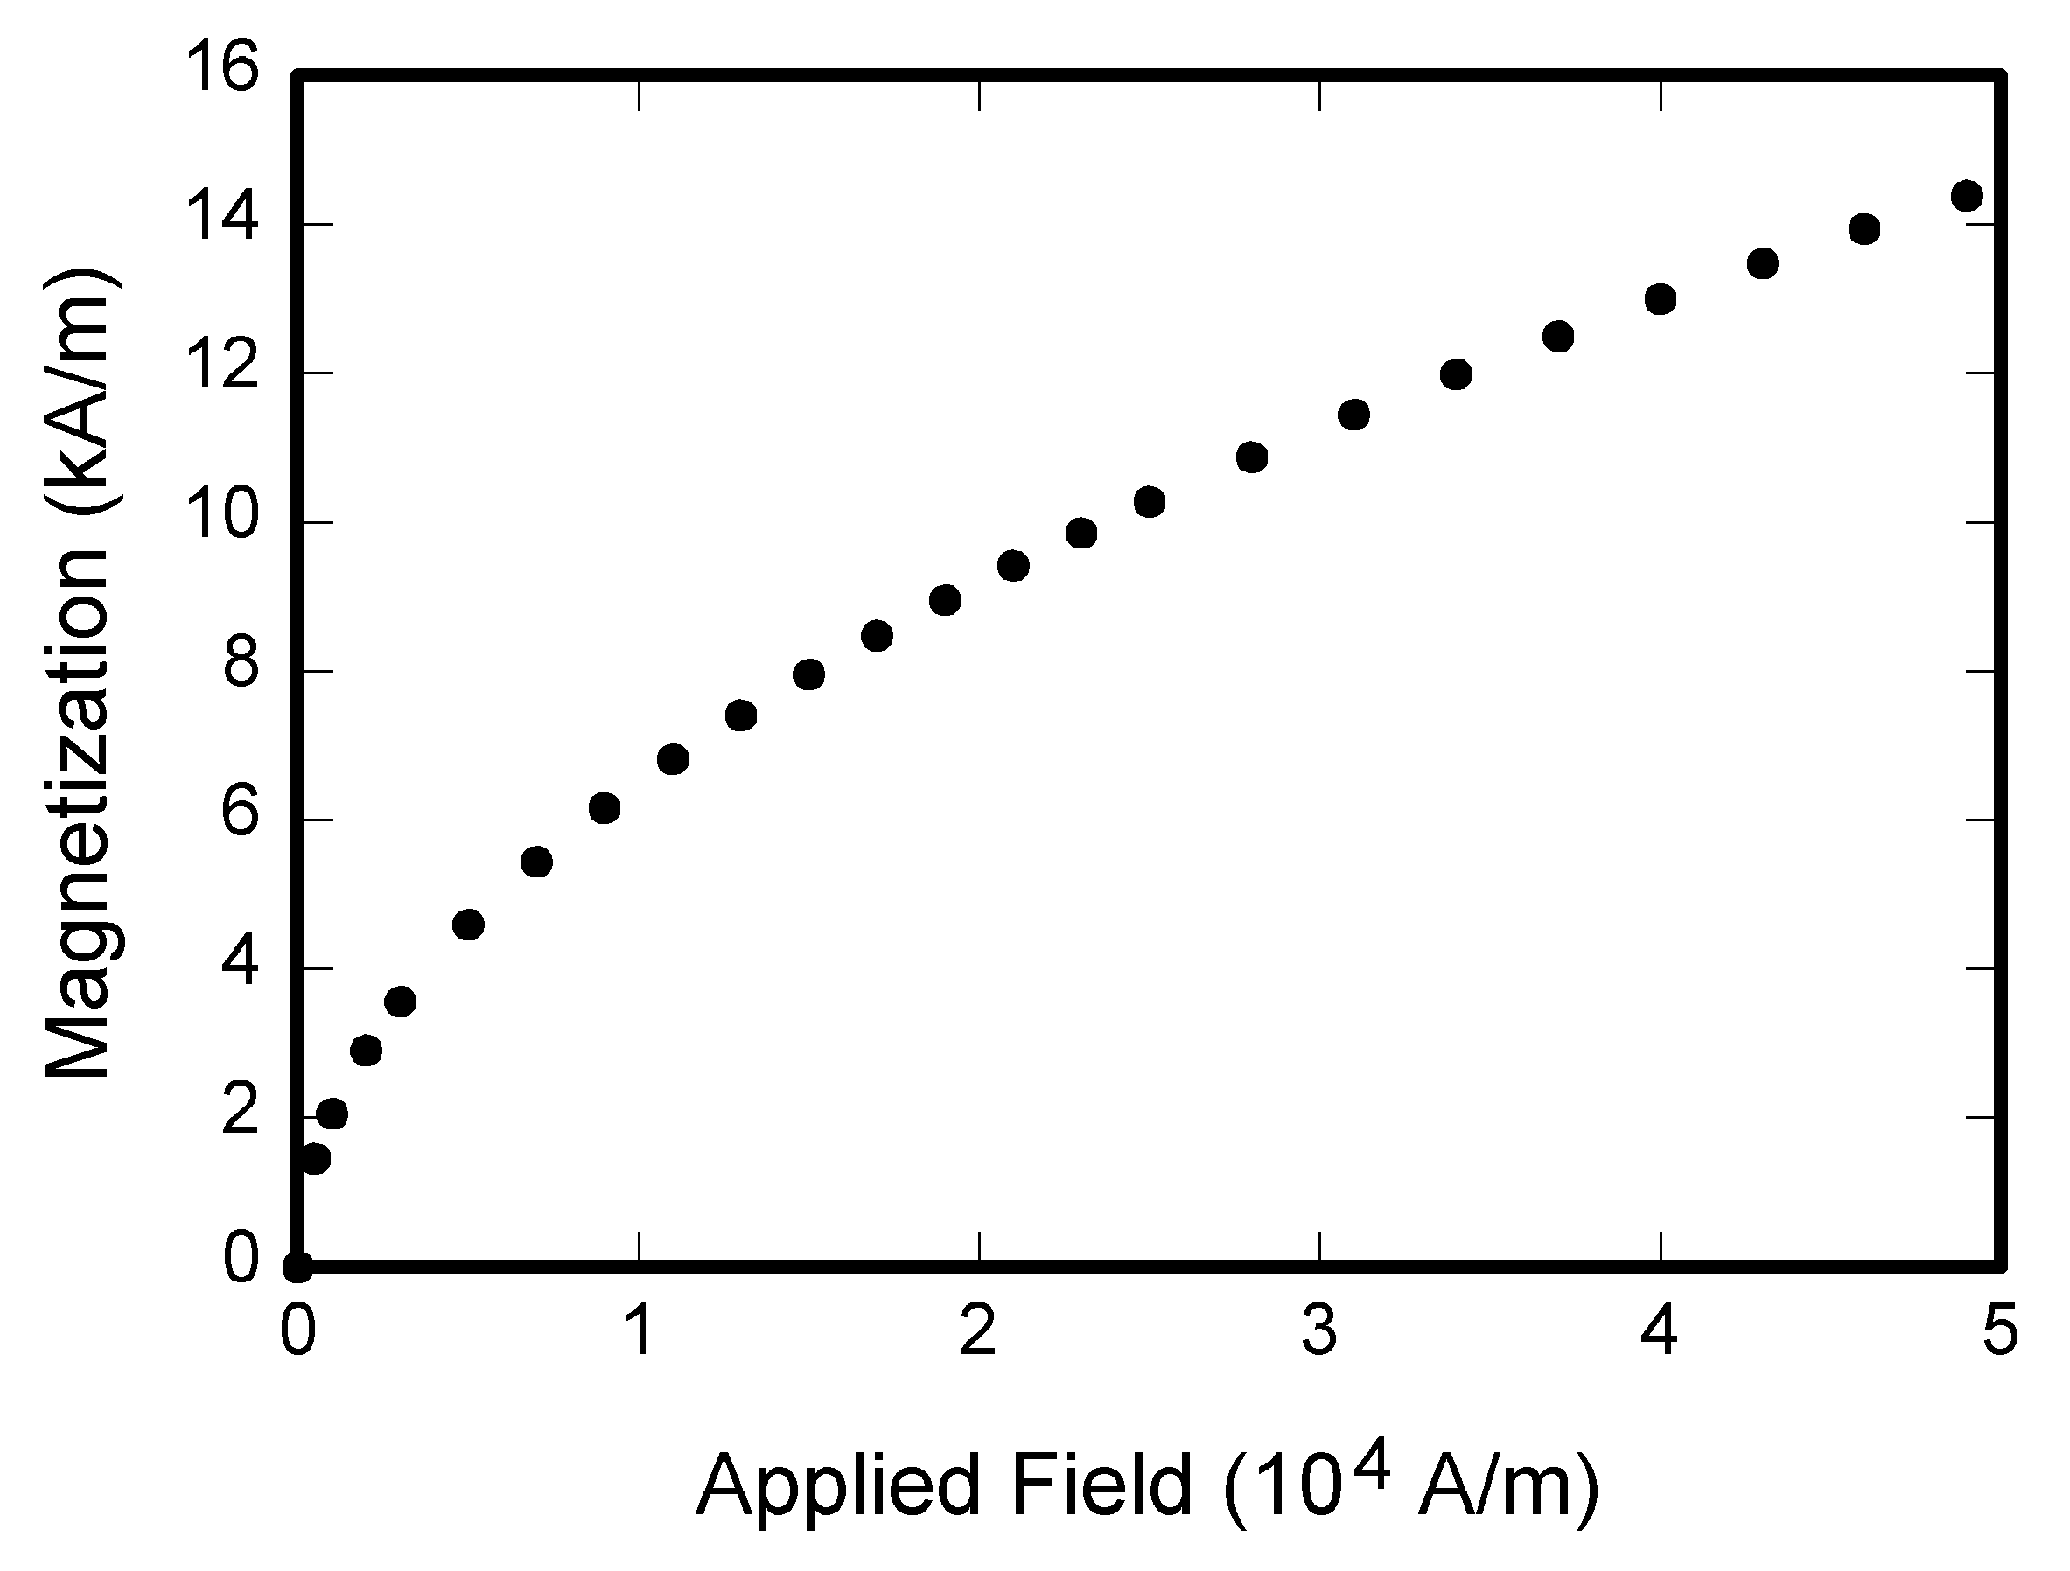
\includegraphics[width=18.5pc]{fig/fig1.png}}
\caption{Map of Antarctic basins used for dedrafting}
\end{figure}

\begin{figure}
\centerline{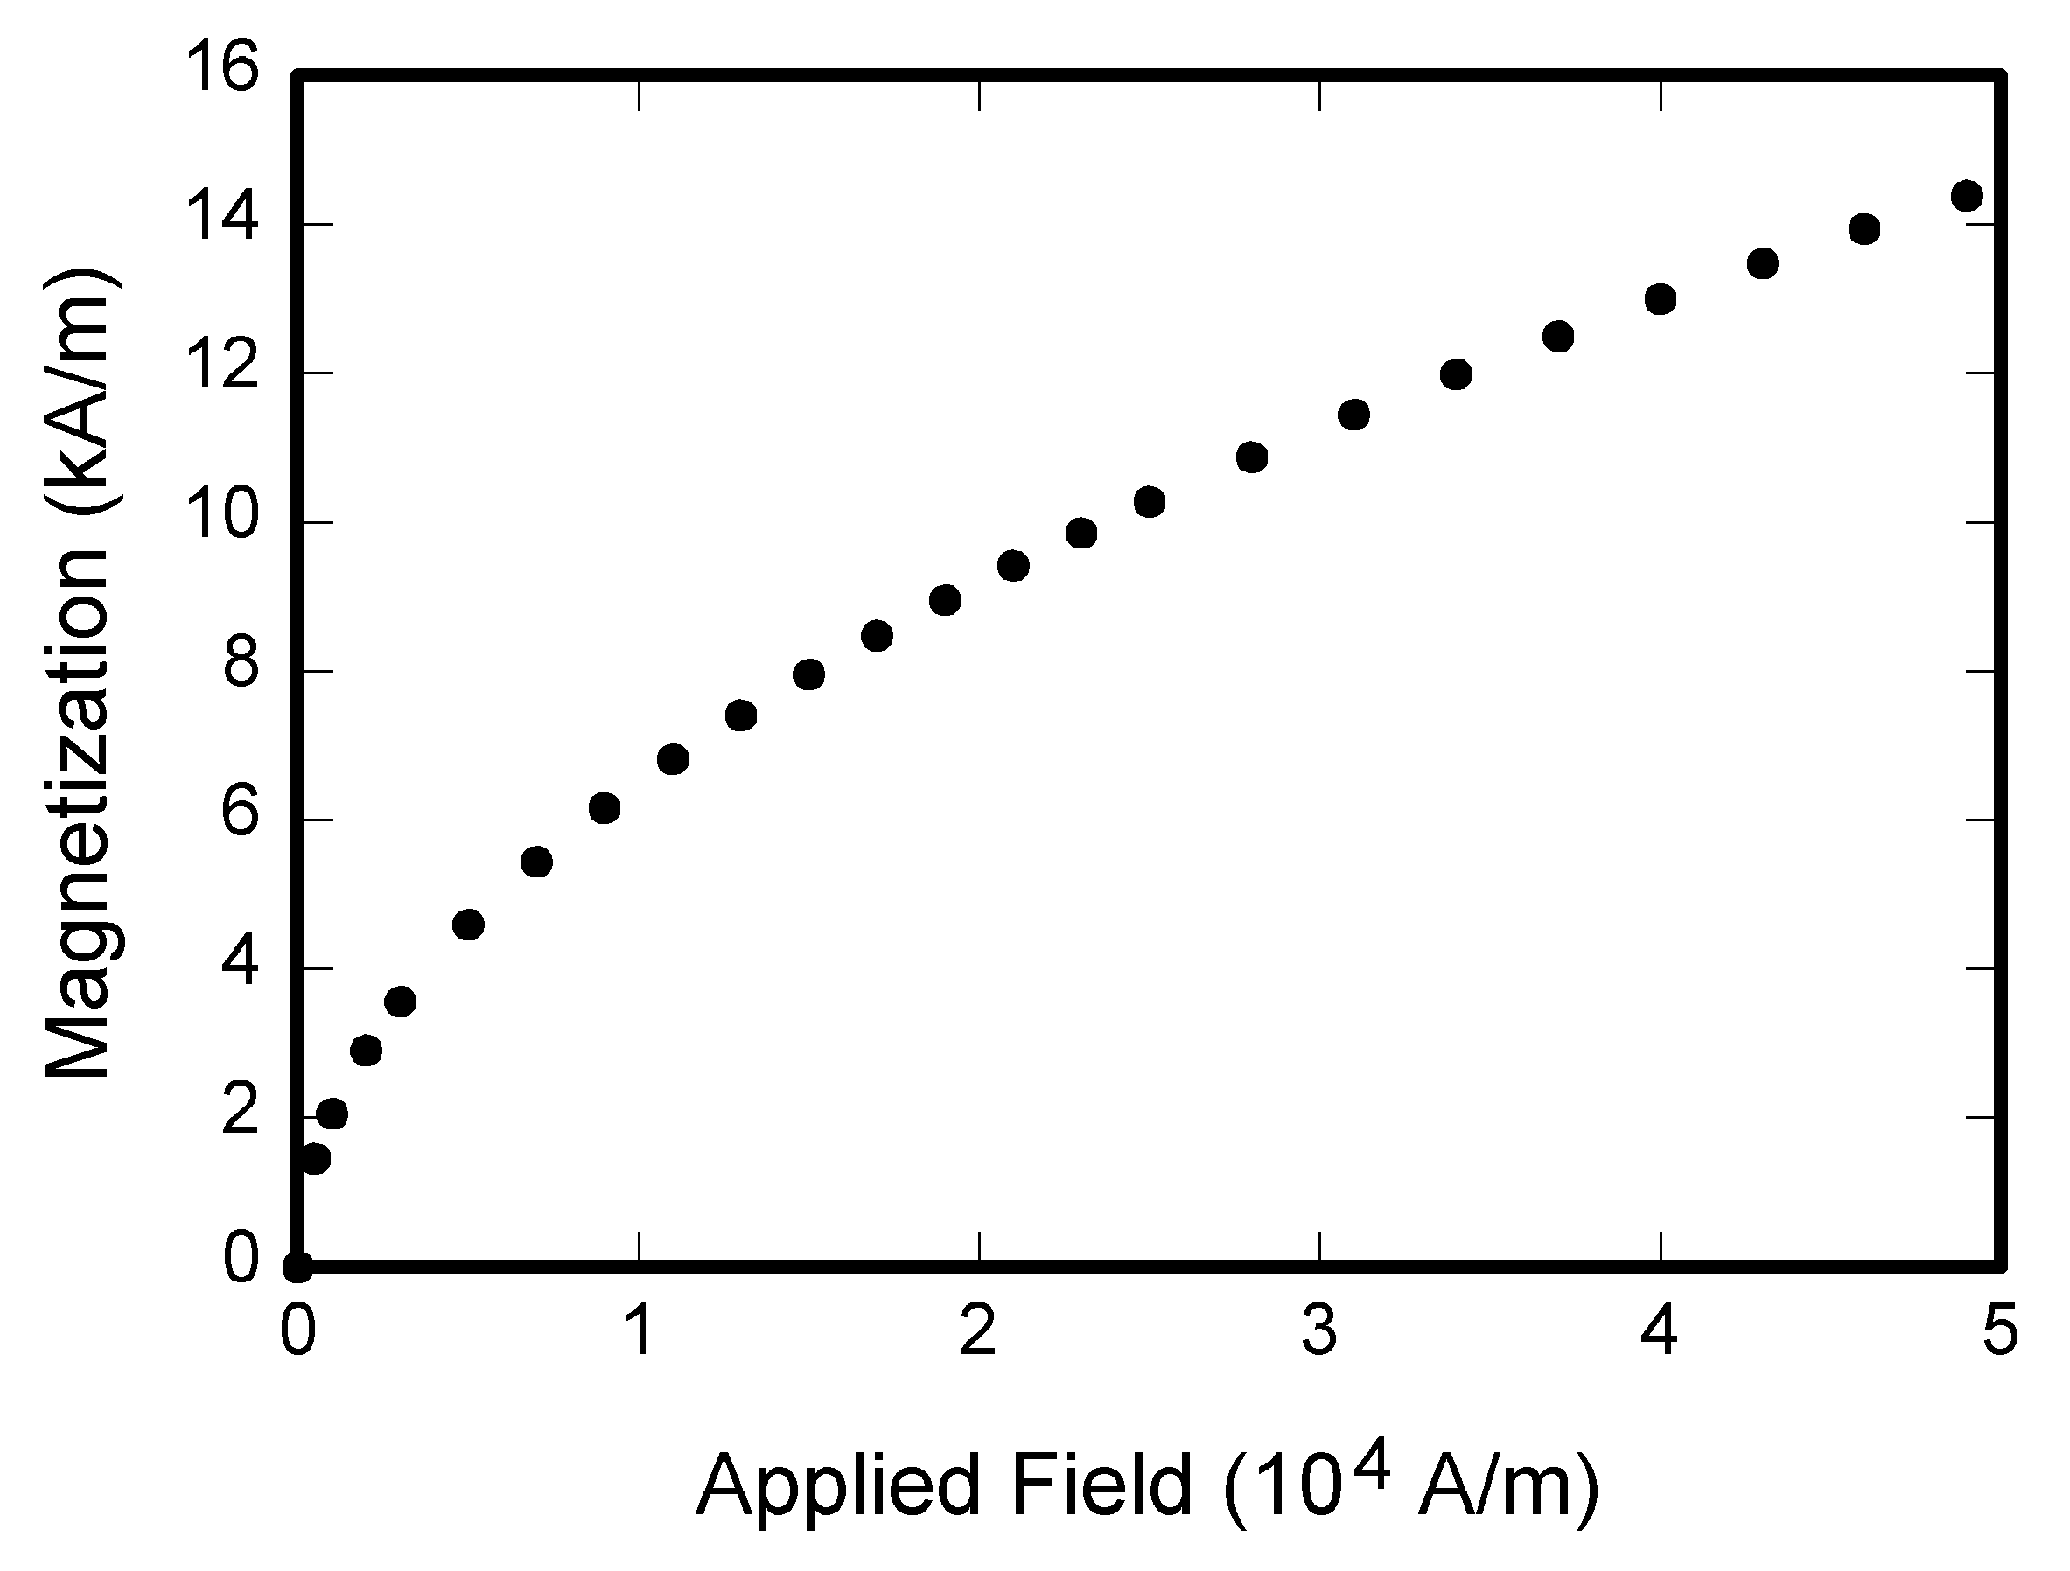
\includegraphics[width=18.5pc]{fig/fig1.png}}
\caption{Melt-draft relationship for different ice shelves, seasonality - can this be an inset?}
\end{figure}

\begin{figure}
\centerline{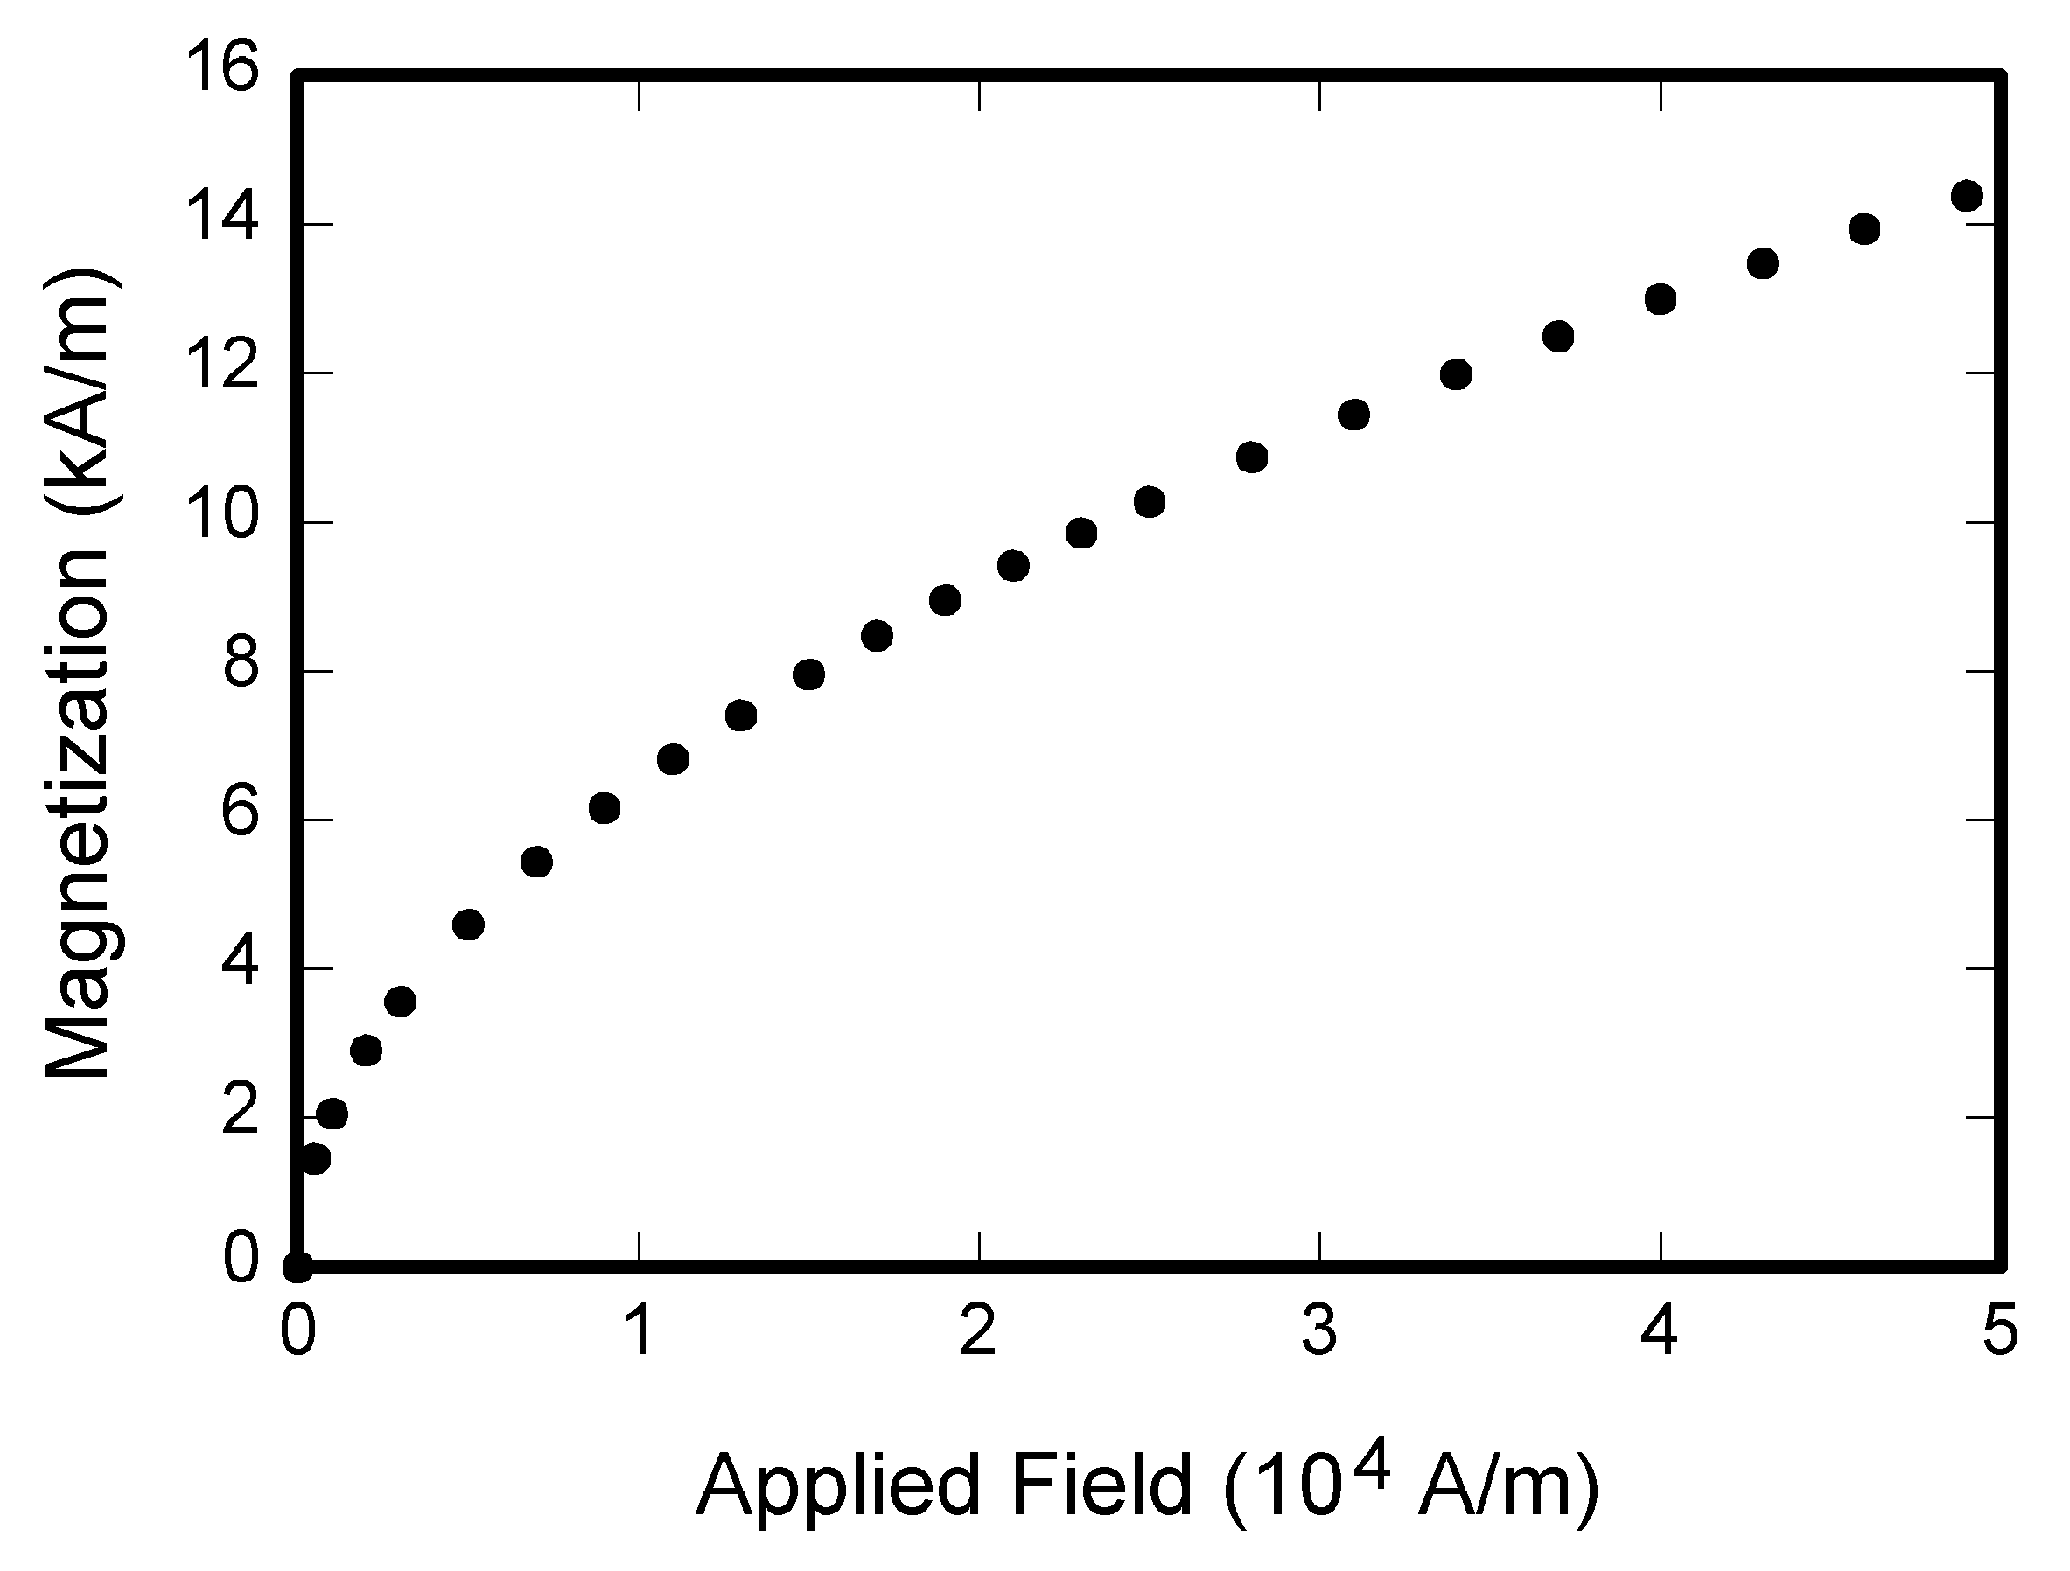
\includegraphics[width=18.5pc]{fig/fig1.png}}
\caption{correlation analyses within and across ice shelves}
\end{figure}

\begin{figure}
\centerline{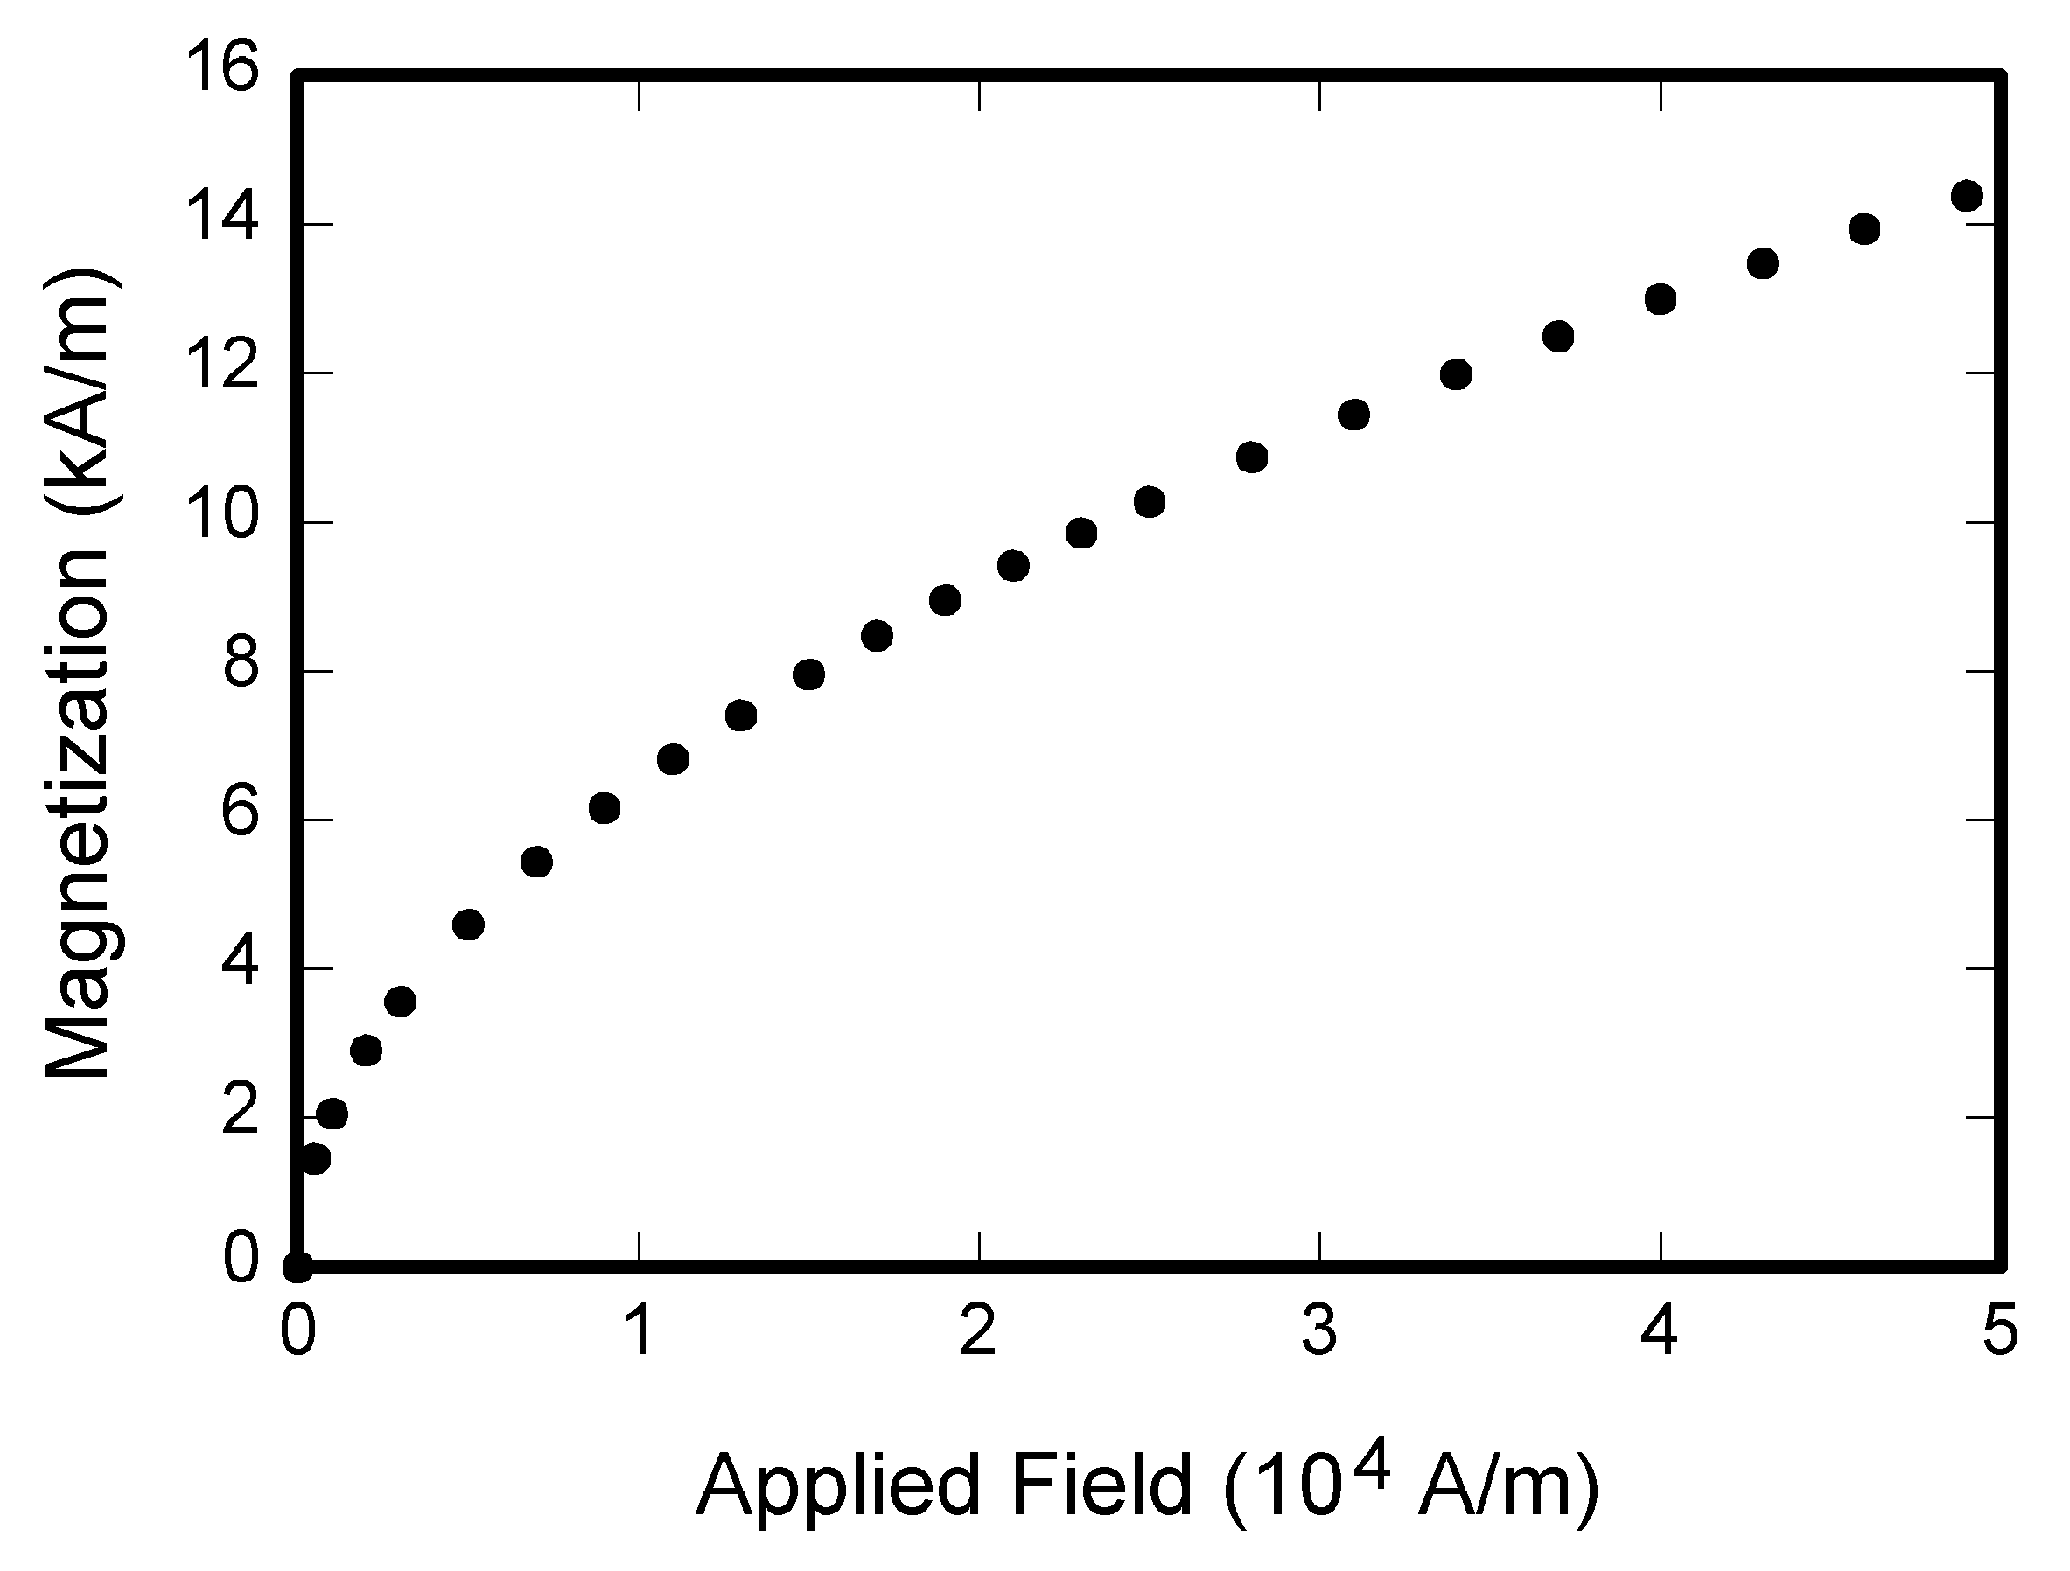
\includegraphics[width=18.5pc]{fig/fig1.png}}
\caption{regional split of basins}
\end{figure}

Decomposition:
	1. Relative power of EOFs in spatial decomposition + Sample maps of EOFs (how many?)
	2. Projection co-efficient PSDs? (to showcase most dominant temporal modes) 
5. Generator:
	1. Phase randomized projection co-efficients for ensemble of realizations
	2. Generated realizations - Power Spectral Densities comparison (specific basins of interest? Amery, Filchner-Ronne, Ross/Thwaites)